\subsection{Zählrohr-Charakteristik}
Für die Zählrohr-Charakteristik werden in Zeitintervallen von $\Delta t = \SI{10}{\second} $ Impulse (Counts) $N$  für verschiedene angelegte Spannungen gemessen. Die Zählrate $Z$ entspricht der Anzahl der Pulse pro Sekunde. Der Fehler der statistischen Poisson-Verteilung ist  
\begin{align*}
	\sigma_N &= \sqrt{N}  \\
	\Rightarrow \sigma_Z &= \sqrt{N}/\Delta t \quad .
\end{align*}	
Die Messdaten (siehe Tabelle~\ref{tab:charakteristik}) sind in Abbildung~\ref{fig:charakteristik_gesamt} dargestellt.
	
	 \begin{figure}[h!]
	 	\centering
	 	\captionof{table}{Daten der Zählrohr-Charakteristik}
	 	\begin{tabular}{ccc|ccc}
	 		$U \ /\  \mathrm{V}$ &$Z \ /\ {\mathrm{Counts}}/{\mathrm{s}}$ & $\Delta Z \ /\ {\mathrm{Counts}}/{\mathrm{s}}$& $U \ /\  \mathrm{V}$ & $Z \ /\ {\mathrm{Counts}}/{\mathrm{s}}$ & $\Delta Z \ /\ {\mathrm{Counts}}/{\mathrm{s}}$ \\
	 		\hline
	 		\input{build/tabelle_charakteristik.txt}
	 	\end{tabular}
	 	\label{tab:charakteristik}
	 \end{figure}
	 
	 \clearpage

\begin{figure}[h!]
	\centering
	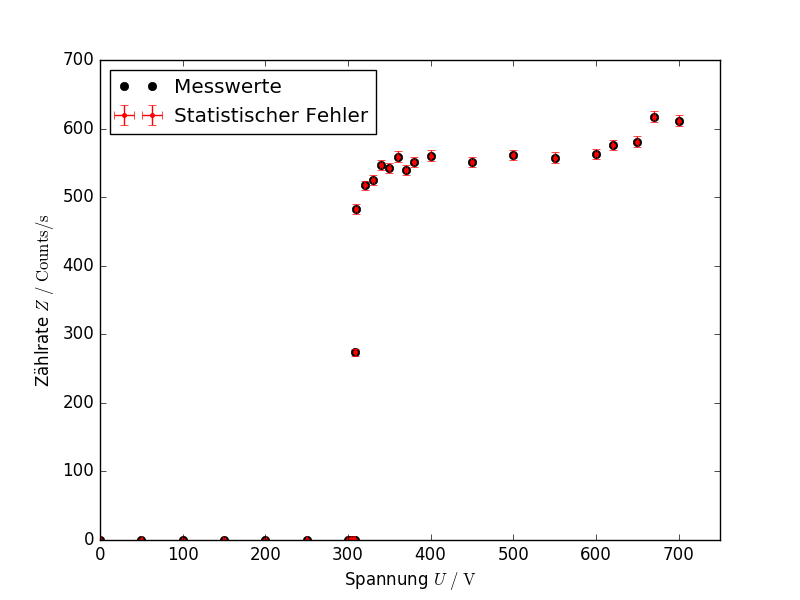
\includegraphics[width=0.8\textwidth]{build/charakteristik_gesamt.png}
	\caption{Alle Messdaten Zählrohr-Charakterisitk}
	\label{fig:charakteristik_gesamt}
\end{figure}



\begin{figure}[h!]
	\centering
	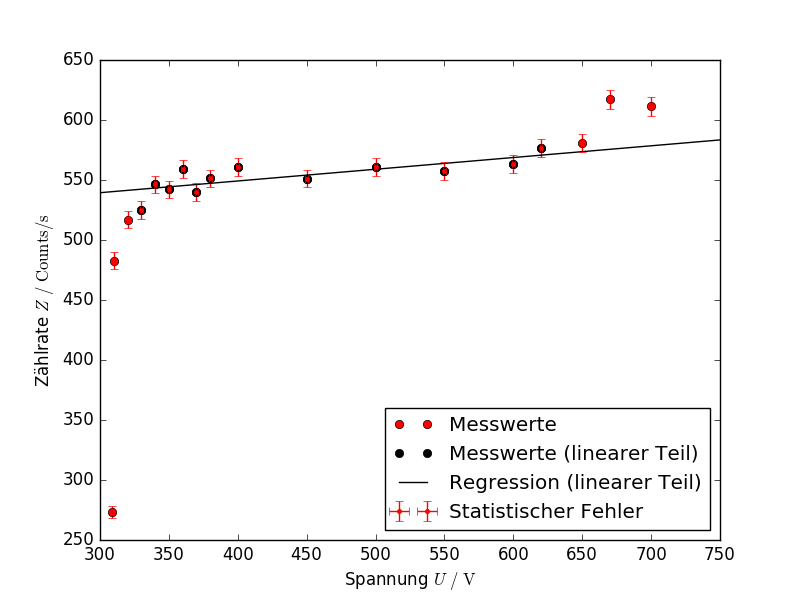
\includegraphics[width=0.8\textwidth]{build/charakteristik_linear.png}
	\caption{Regression an den linearen Anteil der Messdaten der Zählrohr-Charakterisitk. Die ausgenommenen Datenpunkte sind rot gekennzeichnet und die Daten, die in der Regression berücksichtigt sind, schwarz.}
	\label{fig:charakteristik_linear}
\end{figure}

\clearpage
Die Steigung des Plateaus wird mit Hilfe einer Regression an den linearen Teil der Messdaten (siehe Abbildung~\ref{fig:charakteristik_linear}) ermittelt. Die Regression wird mit Hilfe der Pythonversion 3.5.1 durchgeführt. Für die Regressionsvorschrift
\begin{align*}
	Z = m \cdot U +b
\end{align*}
folgen die Fit-Parameter
\begin{align}
	m &= \input{build/m1.txt}\quad , \\
	b &= \input{build/b1.txt} \quad .
\end{align}
Die Steigung $s$ soll nun in $\si{\percent}}/\SI{100}{\volt}$ angegeben werden.
\begin{align}
	s = 100 \cdot \frac{Z_2 - Z_1}{Z_A} \cdot \frac{\si{\percent}}{\SI{100}{\volt}}
\end{align}
Hierbei entspricht $Z_A$ dem Wert der linearen Regression an der Stelle $U_A$, der Mitte des Plateaus, $Z_1$ dem Wert an der Stelle $U_A - \SI{50}{\volt}$ und $Z_2$ dem Wert zu $U_A + \SI{50}{\volt}$.